\documentclass[a4paper, 12pt]{article}
\usepackage[total={17cm,25cm}, top=2.5cm, left=2.5cm, right=2.5cm,  includefoot]{geometry}
\usepackage[utf8]{inputenc}
\usepackage{array}
\usepackage{multirow}
\usepackage{hhline}
\usepackage{gensymb}
\usepackage{graphicx}
\graphicspath{ {} }
\usepackage[czech]{babel}
\usepackage{enumitem}
\usepackage{pdfpages}
\usepackage{amsmath}
\usepackage{verbatim}
\usepackage{listings}
\usepackage{hyperref}
\usepackage{amssymb}


\pagestyle{empty} % vypne číslování stránek




\usepackage[OT2,OT1]{fontenc}
\newcommand\cyr
{
\renewcommand\rmdefault{wncyr}
\renewcommand\sfdefault{wncyss}
\renewcommand\encodingdefault{OT2}
\normalfont
\selectfont
}
\DeclareTextFontCommand{\textcyr}{\cyr}
\def\cprime{\char"7E }
\def\cdprime{\char"7F }
\def\eoborotnoye{\char’013}
\def\Eoborotnoye{\char’003}
\setlength{\parindent}{1em} 
%\setlength{\parskip}{0.5ex}


\begin{document}

\begin{titlepage}
\begin{center}
\Huge
\vspace*{4.5cm}
Algoritmy v digitální kartografii\\
\vspace{0.2cm}

\Large  
Množinové operace s polygony\\
\vspace{0.2cm}

\normalsize  
Zimní semestr 2018/2019\\
%(oprava: 24. 11. 2018)
\vspace{14cm}
\end{center}

\begin{flushright}
\Large
Tereza Kulovaná \\
Markéta Pecenová \\
\end{flushright}

\end{titlepage}


\pagestyle{plain}     % zapne obyčejné číslování
\setcounter{page}{1}  % nastaví čítač stránek znovu od jedné

\tableofcontents
\newpage

\section{Zadání}
Zadání úlohy bylo staženo ze stránek předmětu \href{https://web.natur.cuni.cz/~bayertom/index.php/teaching/algoritmy-v-digitalni-kartografii}{155ADKG}.

\begin{figure}[h!]
	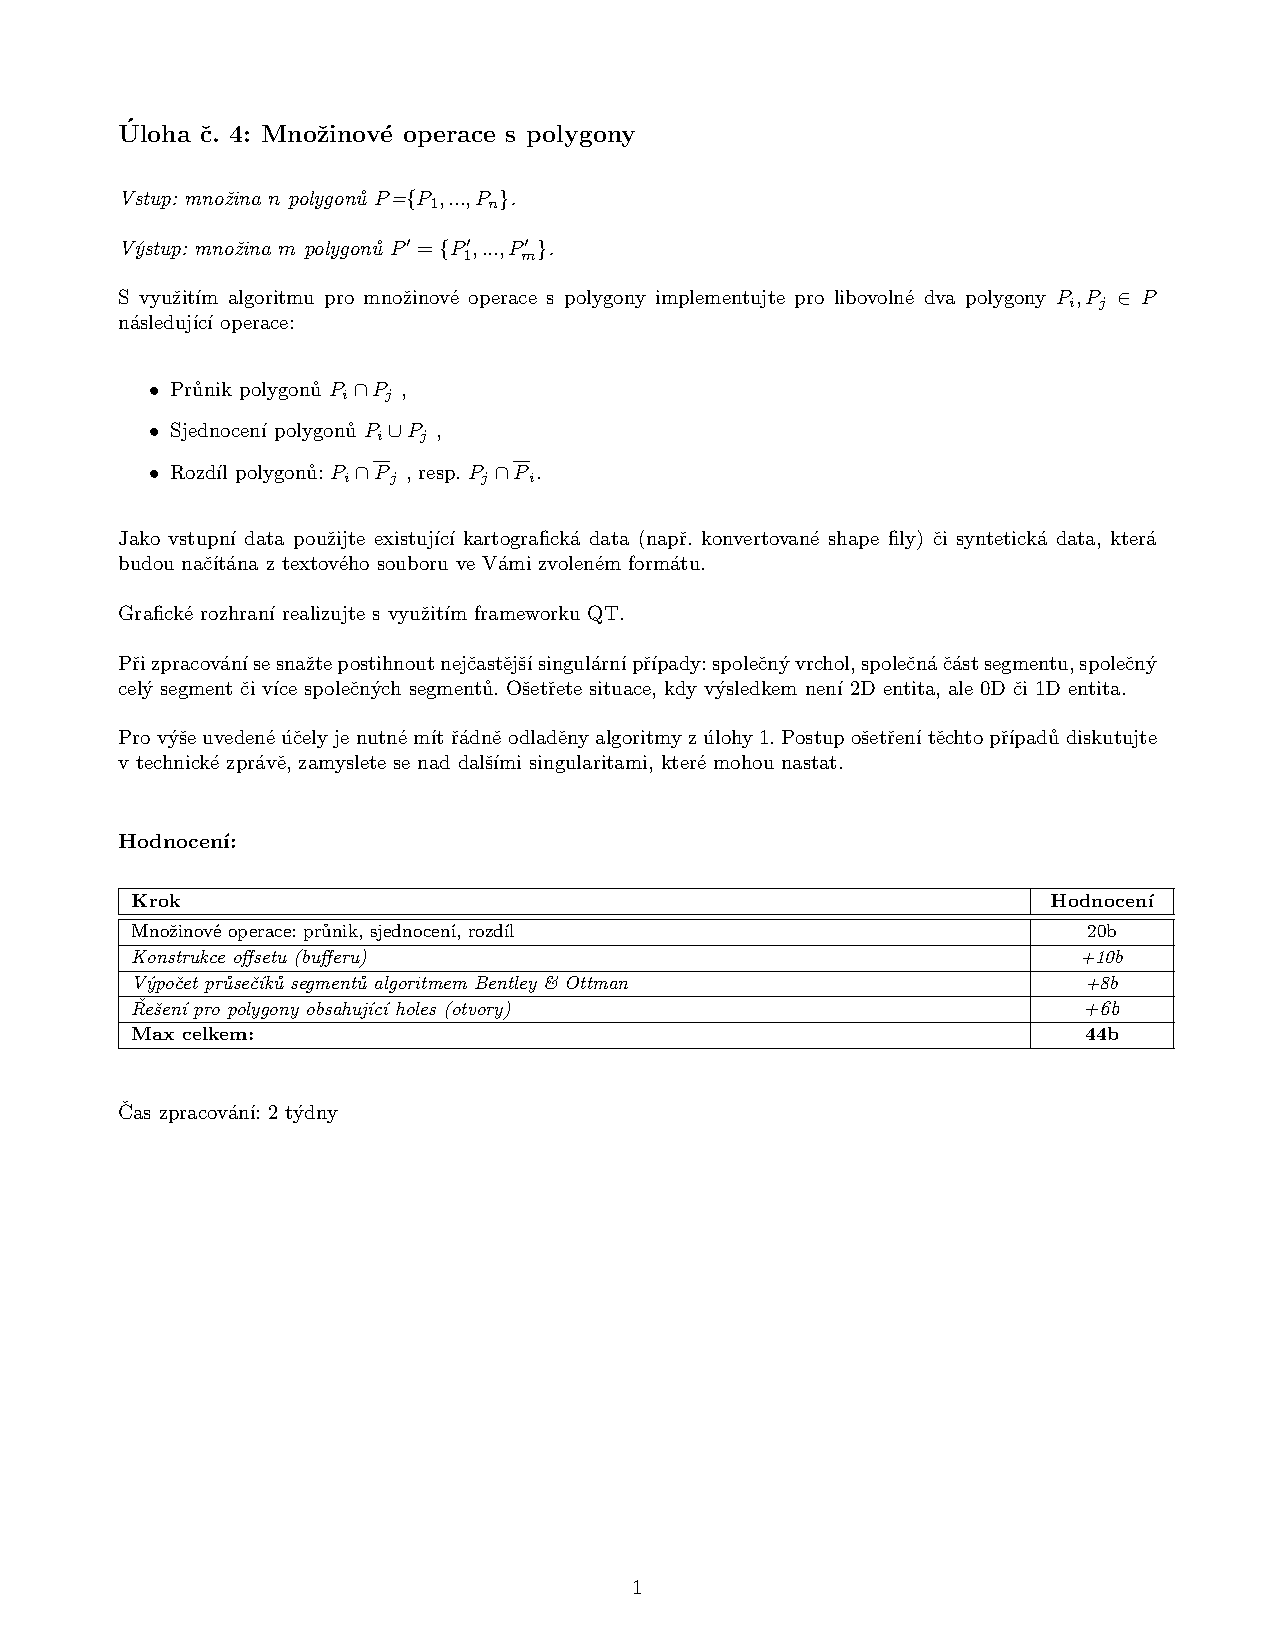
\includegraphics[clip, trim=0cm 8.5cm 0cm 3cm, width=1.0\textwidth]{./pictures/zadani04.pdf}
\end{figure}

V rámci této úlohy nebyly implementovány žádné bonusové úlohy.
\clearpage

\section{Popis a rozbor problému}
Úloha \textbf{Množinové operace s polygony} se zabývá vytvořením aplikace, která nad libovolnými dvěma vstupními polygony provede zvolenou množinovou operaci. 

Mějme vstupní polygony $A$ a $B$. Množinové operace, které nad nimi lze vykonat, jsou následující:
\begin{enumerate}
\item Průnik (Intersection): $\longrightarrow A \cap B$
\item Sjednocení (Union) $\longrightarrow A \cup B$
\item Rozdíl (Difference) $\longrightarrow A$\textbackslash $B$ nebo $B$\textbackslash $A$
\end{enumerate}

\begin{figure}[h!]
	\centering
	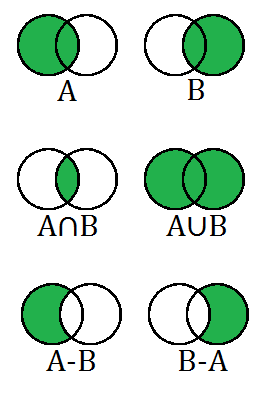
\includegraphics[width=6cm]{./pictures/operations.png}
	\caption{Ukázka množinových operací [\href{http://www.efgh.com/math/algebra/sets.htm}{Zdroj}]}
\end{figure}

\section{Algoritmy}
Tato kapitola se zabývá popisem algoritmů, které byly v aplikaci implementovány. Vzhledem k jejich složitosti je popis výsledného algoritmu rozdělen do jednotlivých fází. Výsledný algoritmus, který spojuje všechny kroky dohromady, se nazývá \textit{BooleanOper}. Vstupní polygony $A$ a $B$ jsou reprezentovány kruhovými seznamy s orientací proti směru hodinových ručiček (CCW). Body, které oba polygony tvoří, mají nově vytvořený datový typ \texttt{QPointFB}.

\subsection{Výpočet průsečíků}
\subsubsection{computePolygonIntersections}
dopsat kecy okolo\\
Průsečíky jsou ukládány do proměnné $M$ datového typu \texttt{map}, která funguje na principu hashování. Spolu s výsledkem je ukládán i tzv. klíč, který na něj odkazuje. Za klíč byl zvolen parametr $\alpha$.\\

Po nalezení každého nového průsečíku je nutné aktualizovat stávající seznamy bodů obou polygonů. K tomu slouží lokální procedura \textit{ProcessIntersection}. Parametr $t$ reprezentuje směrnice $\alpha$ nebo $\beta$, parametr $i$ index daného bodu. DO DOKUMENTACE\\

Zjednodušený zápis algoritmů lze zapsat způsobem uvedeným níže:

\begin{enumerate}
\item Postupně pro všechny $p_i \in A$:
\subitem Vytvoř mapu M 
\subitem Postupně pro všechny $p_j \in B$:
\subitem \hspace {0.5cm} Podmínka ($\exists$ průsečík $b_{ij}$):
\subitem \hspace {1cm} Přidej: M[$\alpha_{i}] \leftarrow b_{ij}$
\subitem \hspace {1cm} Zpracuj průsečík pro $B$: \textit{ProcessIntersection($b_{ij}, \beta, B, j$)}
\subitem Podmínka ($M \neq \emptyset$):
\subitem \hspace {0.5cm} Postupně pro všechny $b_{ij} \in M$:
\subitem \hspace {1cm} Nalezni průsečík pro $A$: \textit{ProcessIntersection($b_{ij}, \alpha, A, i$)}
\end{enumerate}
~\\

Lokální procedura \textit{ProcessIntersection($b, t, P, i$)}:
\begin{enumerate}
\item  Podmínka ($|t| < \epsilon)$: 
\subitem Průsečíkem je počáteční bod: $P[i] \leftarrow inters$
\item  Podmínka ($(|t-1| < \epsilon)$:
\subitem Průsečíkem je koncový bod: $P[(i+1)\%m] \leftarrow inters$
\item  Jinak:
\subitem $i = i+1$
\subitem $P \leftarrow (b,i)$
\end{enumerate}

\subsubsection{setPositions}
Všechny vrcholy polygonu A, resp. B (včetně nalezených průsečíků) jsou následně ohodnoceny, zda leží uvnitř, vně nebo na hraně polygonu B, resp. A. Pro všechny hrany $e_i$ jsou vypočteny jejich středy $\bar{p}$, pro které se následně určuje jejich pozice (ohodnocení $g$) vůči druhému polygonu. Tato informace je uložena do počátečního bodu hrany $e_i$ do parametru pozice. K určení pozice bodů vůči polygonu byl použit algoritmus \textit{GetPositionWinding} z úlohy č.~1. Nejprve jsou zpracovány všechny hrany prvního polygonu a stejný postup je analogicky aplikován i pro druhý polygon. \\

Zjednodušený zápis algoritmů lze zapsat způsobem uvedeným níže:
\begin{enumerate}
\item [] Postupně pro všechny $p_i \in A$:
\subitem $\bar{p} = \frac{p_i(x,y)+p_{i+1}(x,y)}{2}$
\subitem pozice = \textit{GetPositionWinding($\bar{p},B$)}
\subitem $p_i[pozice]$ = pozice
\end{enumerate}

\subsection{Fragmenty}
Sousedící vrcholy se stejným ohodnocením jsou uloženy do samostatných fragmentů $f$. Seznam bodů každého fragmentu začíná průsečíkem a končí bodem s jiným ohodnocením. Pro odlišení je orientace vrcholů ve fragmentech po směru hodinových ručiček (CW). 

\subsubsection{createFragments}
Do metody vstupuje polygon $P$ o velikosti $n$, ohodnocení vrcholů $g$ a seznam fragmentů $F$. Algoritmus obsahuje lokální proceduru \textit{createFragmentFromVertices}, která ze sousedících bodů o stejném ohodnocení vytváří fragment $f$. $i_s$ je index počátečního bodu fragmentu, $i$ je index přidávaného bodu a $g$ ohodnocení.\\

Zjednodušený zápis algoritmů lze zapsat způsobem uvedeným níže:
\begin{enumerate}
\item Inicializace: $i = n-1;~i_s = -1$
\item Dokud ($i > 0$)
\subitem Podmínka ($P[i] =$ průsečík $\land~g(P[i]) = g$)
\subitem \hspace {0.5cm} $i_s = i$; $i--$ 
\item Podmínka ($i_s < 0$) $\rightarrow$ žádný bod neexistuje, ukonči proces
\item Inicializace: $i = i_s$
\item Proveď: 
\subitem Podmínka ($P[i] =$ průsečík $\land~g(P[i]) = g$)
\subitem \hspace {0.5cm} Vytvoř fragment $f = \emptyset$ 
\subitem \hspace {0.5cm} Podmínka (\textit{createFragmentFromVertices} vytvořen)
\subitem \hspace {1cm} Je-li potřeba, prohoď orientaci
\subitem \hspace {1cm} Přidej $f$ do seznamu fragmentů $F$: $F[f[0]] \leftarrow f$
\subitem Jinak inkrementace: $i = (i+1)\%n$
\item[] Dokud ($i \neq i_s$)
\end{enumerate}
~\\

Lokální procedura \textit{createFragmentFromVertices($i_s, P, g, i, f$)}:
\begin{enumerate}
\item[] Opakuj:
\subitem Přidej bod do fragmentu: $f \leftarrow P[i]$
\subitem Inkrementace: $i = (i+1)\%n$
\subitem Podmínka ($i = i_s$) $\rightarrow$ return FALSE
\subitem Podmínka ($g(P[i]) \neq g$)
\subitem \hspace {0.5cm} Přidej bod do fragmentu: $f \leftarrow P[i]$
\subitem \hspace {0.5cm} Return TRUE
\end{enumerate}

\subsubsection{mergeFragments}
Algoritmus spojuje jednotlivé fragmenty $f$ do výstupních polygonů. Metoda má na vstupu seznam fragmentů $F$ a seznam polygonů $C$, do kterého jsou ukládány výsledné polygony. Metoda nejprve spojí jednotlivé fragmenty do oblastí a ty jsou následně lokální procedurou \textit{createPolygonFromFragments} převedeny na polygony. Počáteční bod fragmentu je značen jako $s$, $n$ značí následující bod.

\begin{enumerate}
\item[] Postupně pro všechna $f \in F$:
\subitem Vytvoř: $P = \emptyset$
\subitem Najdi startovní bod fragmentu: $s = f.first$
\subitem Podmínka ($f$ nebyl ještě zpracován)
\subsubitem Podmínka (\textit{createPolygonFromFragments})
\subsubitem Přidej: $C \leftarrow P$
\end{enumerate}
~\\

Lokální procedura \textit{createPolygonFromFragments($s, F, P$)}:
\begin{enumerate}
\item[] Inicializace: $n = s$
\subitem Opakuj:
\subsubitem Nalezni další fragment: $f = F.find(n)$
\subsubitem Podmínka (fragment s daným počátečním bodem $\nexists$) $\rightarrow$ return FALSE
\subsubitem Označ fragment za zpracovaný: $f.second.first \leftarrow$ TRUE
\subsubitem Nalezni další bod: $n \leftarrow f.second.second.back()$
\subsubitem Přidej ho bez počátečního bodu: $P \leftarrow f.second.second - {f.second.second[0]}$
\subsubitem Podmínka ($n = s$) $\rightarrow$ return TRUE
\end{enumerate}

\subsection{BooleanOper}
Tento algoritmus spojuje všechny výše uvedené kroky. Na vstupu jsou polygony $A$ a $B$ a typ zvolené množinové operace.
\begin{enumerate}
\item Podmínka (orientace $A \lor B \neq$ CCW) $\rightarrow$ prohoď orientaci
\item \textit{computePolygonIntersections($A,B$)}
\item \textit{setPositions($A,B$)}
\item Vytvoř mapu fragmentů $F$
\item Zvolení ohodnocení: $pos1 = (oper \equiv intersection \lor oper \equiv DiffAB?Inner:Outer)$
\subitem \hspace {2.8cm} $pos2 = (oper \equiv intersection \lor oper \equiv DiffBA?Inner:Outer)$
\item Prohození: $swap1 = (oper \equiv DiffAB? : true : false)$
\subitem \hspace {1.2cm} $swap2 = (oper \equiv DiffBA? : true : false)$
\item \textit{CreateFragments (A, pos1, swap1, F)}
\item[] \textit{CreateFragments (B, pos2, swap2, F)}
\item \textit{MergeFragments (A,B,C)}

\end{enumerate}


\section{Vstupní data}
Pro účely této úlohy byla použita data, která byla naměřena v rámci geodetické výuky v terénu v Mariánské u Jáchymova. Souřadnice X a Y byly pro tuto úlohu zredukovány na rozumnou velikost, souřadnice Z byla zachována. Body byly zaměřeny metodou GNSS a totální stanicí a znázorňují tamní louku a část silnice. Seznam vstupních bodů je uložen v textovém souboru testing\_data.txt. Soubor je nutné do aplikace nahrát pomocí tlačítka \textsl{Load points}. Struktura textového souboru je následující:\\

\noindent
\textit{Sloupec 1}: souřadnice X [m]\\
\textit{Sloupec 2}: souřadnice Y [m]\\
\textit{Sloupec 3}: souřadnice Z [m]\\

Po úspěšném/neúspěšném nahrání souboru je uživatel upozorněn hláškou. Uživatel nemůže kliknout na žádné jiné tlačítko pro výpočty, nejsou-li nahrána data (tlačítka jsou zašedivělá). Aplikace dále nedovoluje spustit výpočty, jejichž fungování je závislé na vygenerované trojúhelníkové síti, nebyla-li předtím vytvořena. Uživatel má dále možnost zvolit krok, v jakém se budou vykreslovat vrstevnice. Hodnoty lze měnit šipkami nahoru/dolů po 5 m nebo ručně vepsat hodnotu celého čísla v rozmezí 1 m až 100 m. Delaunayova triangulace, vrstevnice, sklon a orientace se generují stisknutím příslušných tlačítek.

\section{Výstupní data}
Vstupní množina bodů a nad ní vygenerovaná trojúhelníková síť je zobrazena ve grafickém okně aplikace. Vykreslování vrstevnic, sklonu a orientace je odděleno. U vrstevnic je každá pátá (hlavní) zvýrazněna. Sklon je v odstínech šedi (čím vyšší sklon, tím tmavší barva). Pro zobrazení orientace trojúhelníků ke světovým stranám byla využita prostřední kružnice barvené škály ze stránek společnosti \textit{ESRI}, viz níže. Aplikace je uvedena do výchozího stavu stisknutím tlačítka \textsl{Clear}.\\


\clearpage
\section{Aplikace}
V následují kapitole je představen vizuální vzhled vytvořené aplikace tak, jak ji vidí prostý uživatel.

\begin{comment}

\begin{figure}[h!]
	\centering
	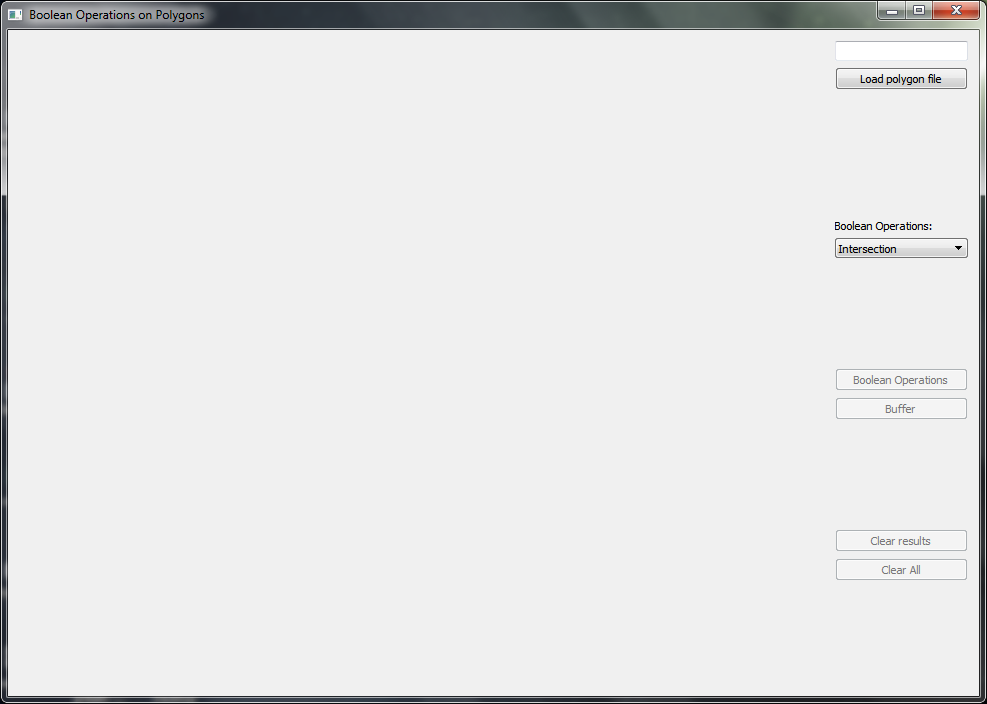
\includegraphics[width=14cm]{./pictures/app_default.png}
	\caption{Výchozí vzhled aplikace po spuštění}
\end{figure}

\begin{figure}[h!]
	\centering
	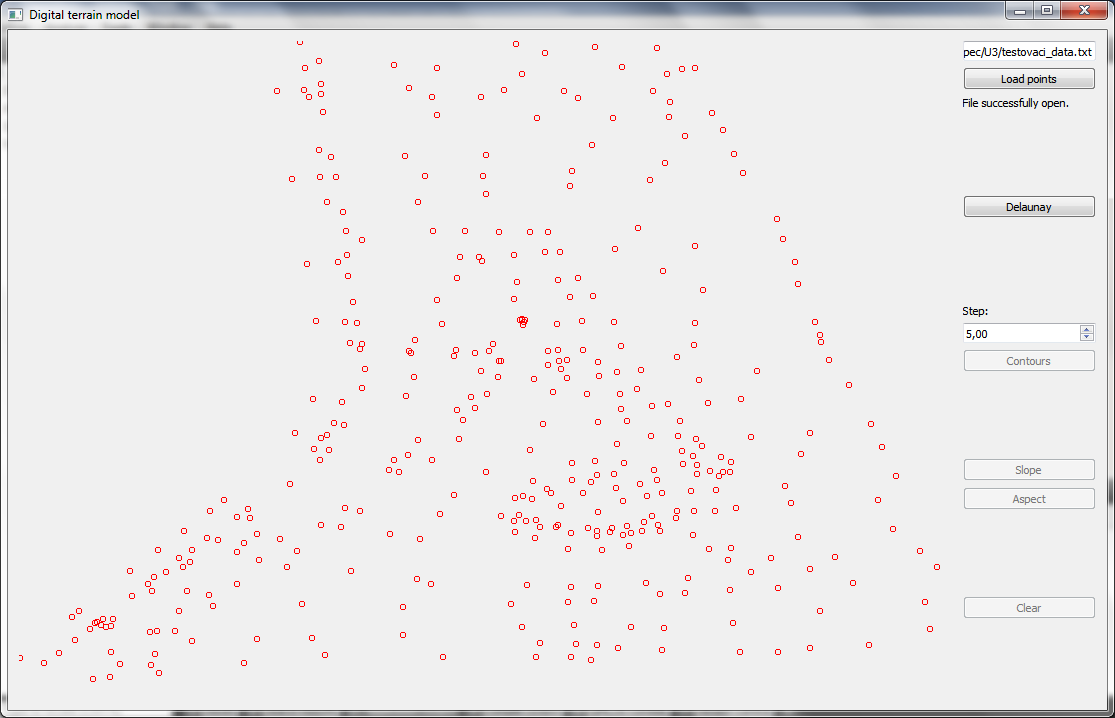
\includegraphics[width=14cm]{./pictures/app_load_points.png}
	\caption{Aplikace po nahrání vstupních dat}
\end{figure}

\begin{figure}[h!]
	\centering
	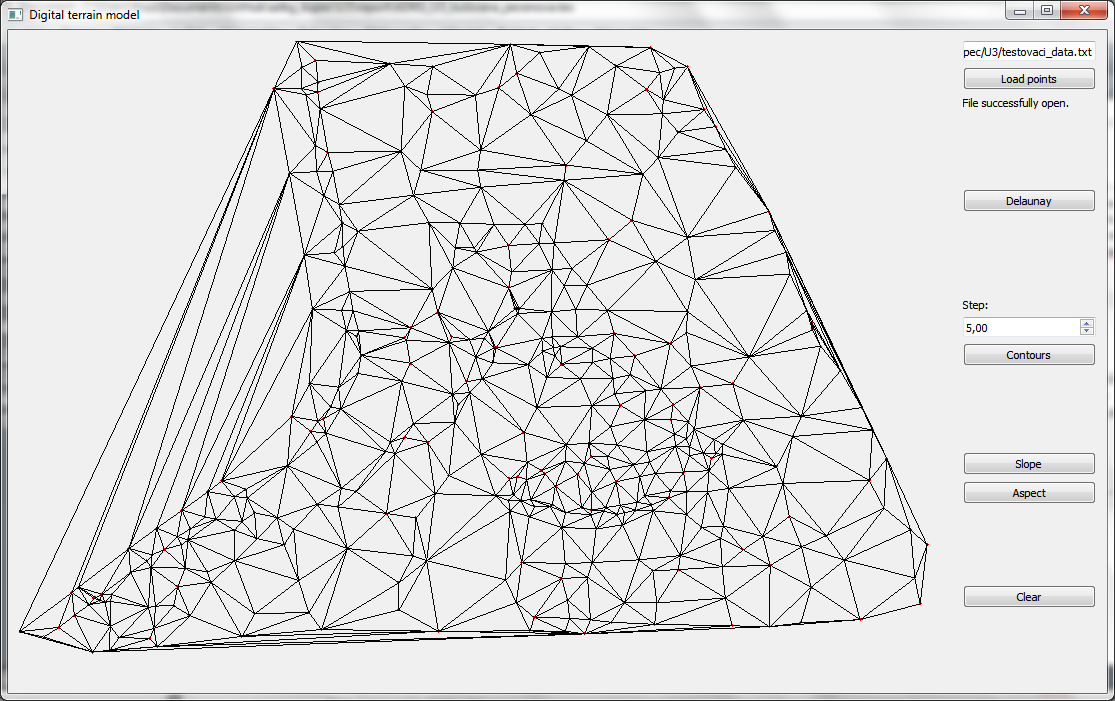
\includegraphics[width=15cm]{./pictures/app_delaunay.png}
	\caption{Trojúhelníková síť}
\end{figure}

\begin{figure}[h!]
	\centering
	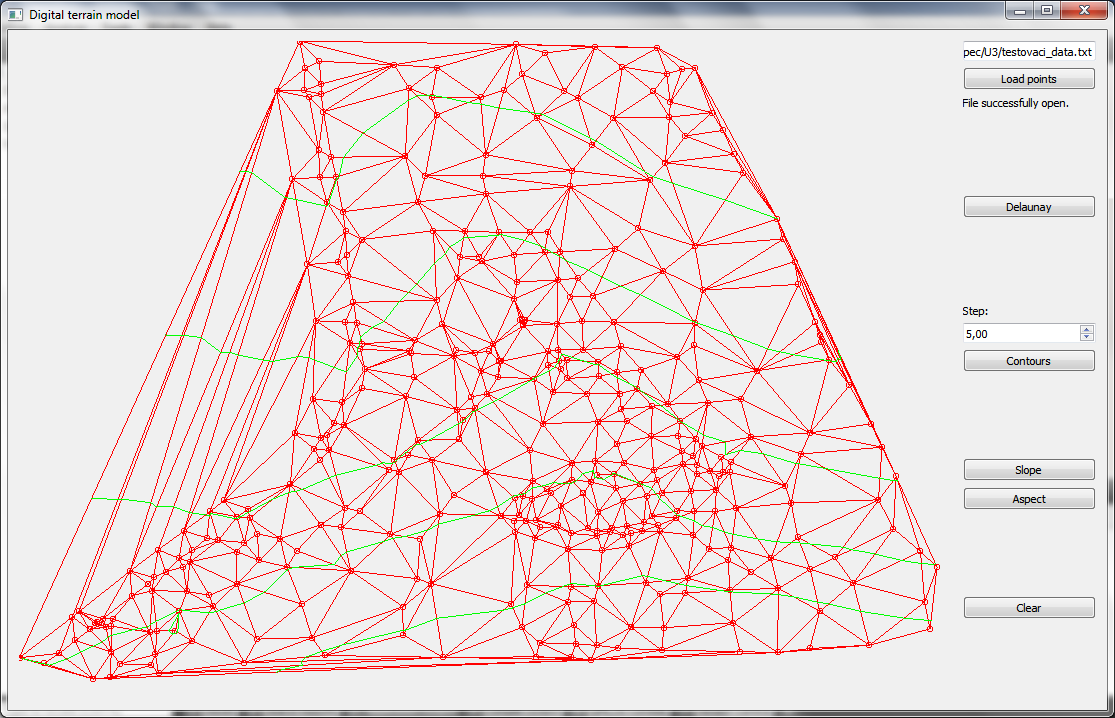
\includegraphics[width=15cm]{./pictures/app_contours.png}
	\caption{Vykreslení vrstevnic}
\end{figure}

\begin{figure}[h!]
	\centering
	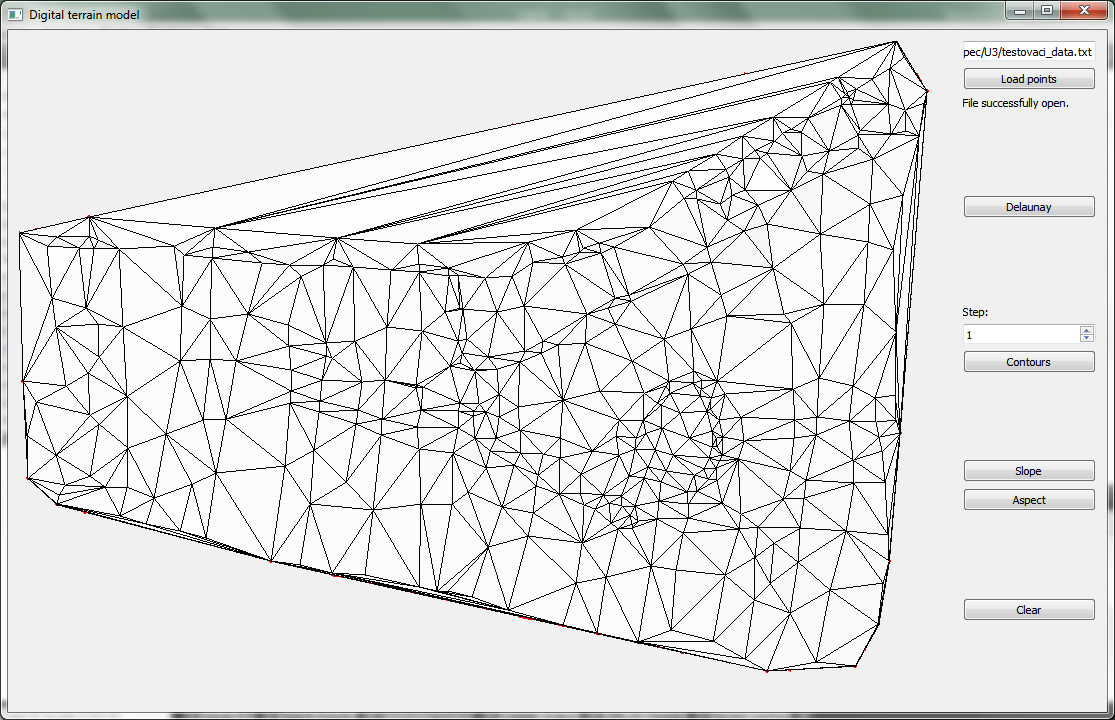
\includegraphics[width=15cm]{./pictures/app_slope.png}
	\caption{Sklon trojúhelníků}
\end{figure}

\begin{figure}[h!]
	\centering
	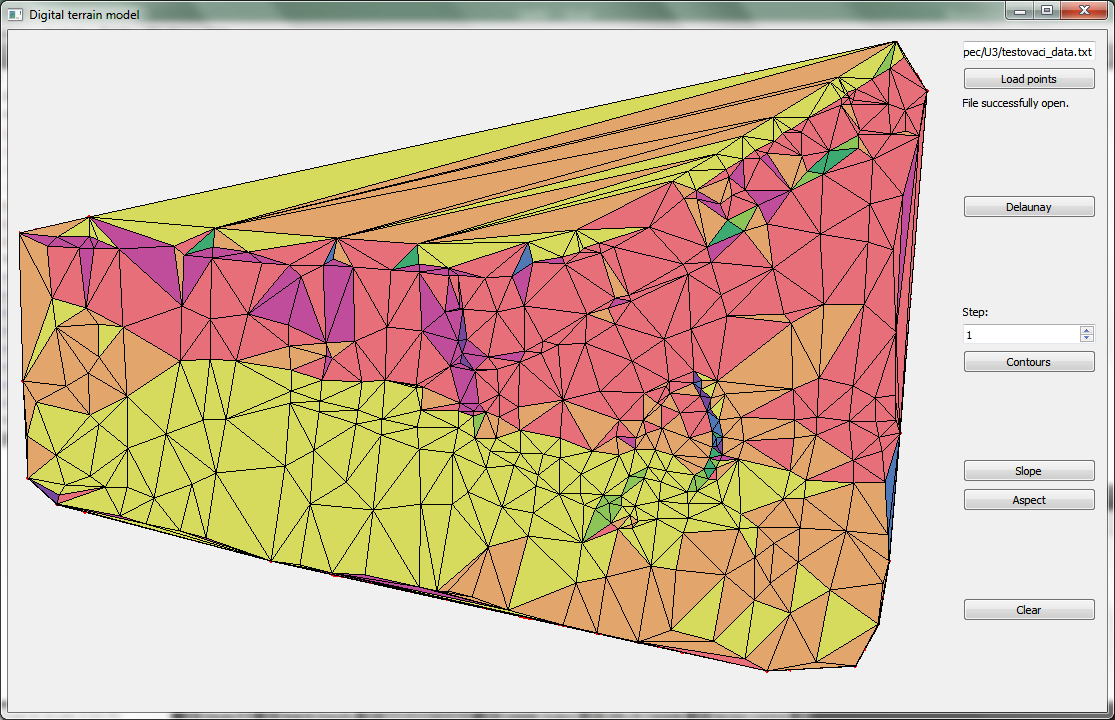
\includegraphics[width=15cm]{./pictures/app_aspect.png}
	\caption{Orientace trojúhelníků}
\end{figure}

\end{comment}
\clearpage


 
\section{Dokumentace}
Tato kapitola obsahuje dokumentaci k jednotlivým třídám.

\subsection{!Algorithms}
Třída \textit{Algorithms} obsahuje metody pro výpočet Delaunayovy triangulace a analýzu DTM.



\subsubsection*{getPositionWinding}
Metoda \textbf{getPositionWinding} určuje polohu bodu $q$ vzhledem k polygonu $P$ za použití algoritmu \textsl{Winding Number}. Na vstupu je bod $q$ a vektor bodů polygonu třídy \texttt{QPointFB}. Návratová hodnota typu \texttt{TPointPolygon} vrací polohu bodu $q$ vůči polygonu $P$.\\

\textbf{Input}:
\begin{itemize}
\item \texttt{QPointFB} $q$
\item \textsl{vector} $\textless$\texttt{QPointFB}$\textgreater$ $P$
\end{itemize}

\textbf{Output}:
\begin{itemize}
\item \texttt{INSIDE} $\rightarrow q$ se nachází uvnitř polygonu $P$
\item \texttt{OUTSIDE} $\rightarrow q$ se nachází vně polygonu $P$
\item \texttt{ON} $\rightarrow q$ se nachází na hraně polygonu $P$
\end{itemize}

\subsubsection*{getPointLinePosition}
Metoda \textbf{getPointLinePosition} určuje polohu bodu $q$ vzhledem k přímce tvořené dvěma body. Na vstupu jsou 3 body typu \texttt{QPointFB}, návratová hodnota je nově definovaný typ \texttt{TPosition}.\\

\textbf{Input}:
\begin{itemize}
\item \texttt{QPointFB} $q$
\item \texttt{QPointFB} $a$
\item \texttt{QPointFB} $b$
\end{itemize}

\textbf{Output}:
\begin{itemize}
\item \texttt{LEFT} $\rightarrow$ bod se nachází vlevo od přímky
\item \texttt{RIGHT} $\rightarrow$ bod se nachází vpravo od přímky
\item \texttt{ON} $\rightarrow$ bod se nachází na přímce
\end{itemize}

\subsubsection*{get2LinesAngle}
Metoda \textbf{get2LinesAngle} počítá úhel mezi dvěma přímkami. Na vstupu jsou 4 body typu \texttt{QPointFB}, návratová hodnota typu \texttt{double} vrací velikost úhlu v radiánech. Body $p_1$ a $p_2$ definují první přímku, zbylé dva body druhou přímku.\\

\textbf{Input}:
\begin{itemize}
\item \texttt{QPointFB} $p_1$ 
\item \texttt{QPointFB} $p_2$ 
\item \texttt{QPointFB} $p_3$
\item \texttt{QPointFB} $p_4$
\end{itemize}

\textbf{Output}:
\begin{itemize}
\item \texttt{double} 
\end{itemize}

\subsubsection*{get2LinesPosition}
Metoda \textbf{get2LinesPosition} určuje vzájemnou polohu dvou přímek. Pokud se přímky protínají, metoda vypočte jejich průsečík $p_{inters}$. Na vstupu jsou 4 body typu \texttt{QPointFB}, návratová hodnota je nově definovaný typ \texttt{T2LinesPosition}. Body $p_1$ a $p_2$ definují první přímku, zbylé dva body druhou přímku.\\

\textbf{Input}:
\begin{itemize}
\item \texttt{QPointFB} $p_1$ 
\item \texttt{QPointFB} $p_2$ 
\item \texttt{QPointFB} $p_3$
\item \texttt{QPointFB} $p_4$
\item \texttt{QPointFB} $p_{inters}$
\end{itemize}

\textbf{Output}:
\begin{itemize}
\item \texttt{PARALLEL} $\rightarrow$ přímky jsou rovnoběžné
\item \texttt{COLINEAR} $\rightarrow$ přímky jsou kolineární
\item \texttt{INTERSECTING} $\rightarrow$ přímky se protínají v průsečíku $p_{inters}$
\item \texttt{NONINTERSECTING} $\rightarrow$ přímky se neprotínají
\end{itemize}

\subsubsection*{computePolygonIntersections}
Metoda \textbf{computePolygonIntersections} počítá průsečíky dvou polygonů $A$ a $B$. Na vstupu jsou dva vektory bodů polygonů, návratová hodnota je typu \texttt{void}.\\

\textbf{Input}:
\begin{itemize}
\item \textsl{vector} $\textless$\texttt{QPointFB}$\textgreater$ $polA$
\item \textsl{vector} $\textless$\texttt{QPointFB}$\textgreater$ $polB$
\end{itemize}

\subsection*{processIntersection}
Metoda \textbf{processIntersection} slouží k aktualizování seznamu bodů (tzv. map) obou polygonů po přidání nově nalezeného průsečíku. Na vstupu je .... Návratová hodnota je typu \texttt{void}.\\

\textbf{Input}:
\begin{itemize}
\item \texttt{QPointFB} $b$
\item \texttt{double} $t$
\item \textsl{vector} $\textless$\texttt{QPointFB}$\textgreater$ $pol$
\item \texttt{int} $i$
\end{itemize}

\subsubsection*{setPositions}
Metoda \textbf{setPositions} počítá orientaci trojúhelníku, který je tvořen třemi body, ke světovým stranám. Návratová hodnota typu \texttt{double} vrací orientaci trojúhelníku ve stupních. Orientace je pravotočivá a nabývá hodnot $\textless$-180$^\circ$;180$^\circ\textgreater$.\\

\textbf{Input}:
\begin{itemize}
\item \texttt{QPoint3D} $p_1$
\item \texttt{QPoint3D} $p_2$
\item \texttt{QPoint3D} $p_3$
\end{itemize}

\subsubsection*{createFragments}
Metoda \textbf{createFragments} vytváří z vektoru hran trojúhelníky a počítá pro ně sklon a orientaci. Vypočtené hodnoty ukládá do datového typu \texttt{Triangle}. Návratová hodnota metody je vektor trojúhelníků typu \texttt{Triangle}.\\

\textbf{Input}:
\begin{itemize}
\item \textsl{vector} $\textless$\texttt{Edge}$\textgreater$ $dt$
\end{itemize}

\textbf{Output}:
\begin{itemize}
\item \textsl{vector} $\textless$\texttt{Triangle}$\textgreater$
\end{itemize}



\subsubsection*{createFragmentFromVertices}
Metoda \textbf{createFragmentFromVertices} počítá poloměr kružnice, která je tvořena 3 body. Na vstupu jsou 4 body typu \texttt{QPoint3D}, návratová hodnota typu \texttt{double} vrací velikost poloměru kružnice.\\ 

\textbf{Input}:
\begin{itemize}
\item \texttt{QPoint3D} $p_1$ 
\item \texttt{QPoint3D} $p_2$ 
\item \texttt{QPoint3D} $p_3$
\item \texttt{QPoint3D} $c \rightarrow$ střed kružnice
\end{itemize}

\subsubsection*{mergeFragments}
Metoda \textbf{mergeFragments} počítá vzdálenost mezi dvěma body. Na vstupu jsou 2 body typu \texttt{QPoint3D}, návratová hodnota typu \texttt{double} vrací vzdálenost mezi dvěma body.\\ 

\textbf{Input}:
\begin{itemize}
\item \texttt{QPoint3D} $p_1$ 
\item \texttt{QPoint3D} $p_2$
\end{itemize}

\subsubsection*{createPolygonFromFragments}
Metoda \textbf{createPolygonFromFragments} slouží k nalezení nejbližšího bodu z množiny bodů vzhledem k danému bodu $p$. Na vstupu je daný bod $p$ a vektor bodů typu \texttt{QPoint3D}. Návratová hodnota typu \texttt{int} vrací index nejbližšího bodu.

\textbf{Input}:
\begin{itemize}
\item \texttt{QPoint3D} $p$ 
\item \textsl{vector} $\textless$\texttt{QPoint3D}$\textgreater$ $points$
\end{itemize}

\subsubsection*{getPolygonOrientation}
Metoda \textbf{getPolygonOrientation} slouží k nalezení třetího bodu trojúhelníku, který splňuje Delaunayovo kritérium nejmenší opsané kružnice. Na vstupu jsou dva body typu \texttt{QPoint3D}, které představují orientovanou hranu, a vektor bodů typu \texttt{QPoint3D}. Návratová hodnota typu \texttt{int} vrací index hledaného bodu.\\

\textbf{Input}:
\begin{itemize}
\item \texttt{QPoint3D} $s$ $\rightarrow$ počáteční bod hrany
\item \texttt{QPoint3D} $e$ $\rightarrow$ koncový bod hrany
\item \textsl{vector} $\textless$\texttt{QPoint3D}$\textgreater$ $points$
\end{itemize}

\subsubsection*{BooleanOper}
Metoda \textbf{BooleanOper} počítá průsečík hrany trojúhelníku tvořené dvěma body typu \texttt{QPoint3D} s rovinou o dané výšce Z. Návratová hodnota je typu \texttt{QPoint3D}.\\

\textbf{Input}:
\begin{itemize}
\item \texttt{QPoint3D} $p_1$ 
\item \texttt{QPoint3D} $p_2$ 
\item \texttt{double} $z$ 
\end{itemize}

\subsubsection*{resetIntersections}
Metoda \textbf{resetIntersections} vytváří z vektoru hran trojúhelníky a počítá pro ně sklon a orientaci. Vypočtené hodnoty ukládá do datového typu \texttt{Triangle}. Návratová hodnota metody je vektor trojúhelníků typu \texttt{Triangle}.\\

\textbf{Input}:
\begin{itemize}
\item \textsl{vector} $\textless$\texttt{Edge}$\textgreater$ $dt$
\end{itemize}

\textbf{Output}:
\begin{itemize}
\item \textsl{vector} $\textless$\texttt{Triangle}$\textgreater$
\end{itemize}

\subsubsection*{lineOffset}
Metoda \textbf{lineOffset} vytváří z vektoru hran trojúhelníky a počítá pro ně sklon a orientaci. Vypočtené hodnoty ukládá do datového typu \texttt{Triangle}. Návratová hodnota metody je vektor trojúhelníků typu \texttt{Triangle}.\\

\textbf{Input}:
\begin{itemize}
\item \textsl{vector} $\textless$\texttt{Edge}$\textgreater$ $dt$
\end{itemize}

\textbf{Output}:
\begin{itemize}
\item \textsl{vector} $\textless$\texttt{Triangle}$\textgreater$
\end{itemize}

\subsubsection*{lineOffset}
Metoda \textbf{lineOffset} vytváří z vektoru hran trojúhelníky a počítá pro ně sklon a orientaci. Vypočtené hodnoty ukládá do datového typu \texttt{Triangle}. Návratová hodnota metody je vektor trojúhelníků typu \texttt{Triangle}.\\

\textbf{Input}:
\begin{itemize}
\item \textsl{vector} $\textless$\texttt{Edge}$\textgreater$ $dt$
\end{itemize}

\textbf{Output}:
\begin{itemize}
\item \textsl{vector} $\textless$\texttt{Triangle}$\textgreater$
\end{itemize}

\subsubsection*{sampleArc}
Metoda \textbf{sampleArc} vytváří z vektoru hran trojúhelníky a počítá pro ně sklon a orientaci. Vypočtené hodnoty ukládá do datového typu \texttt{Triangle}. Návratová hodnota metody je vektor trojúhelníků typu \texttt{Triangle}.\\

\textbf{Input}:
\begin{itemize}
\item \textsl{vector} $\textless$\texttt{Edge}$\textgreater$ $dt$
\end{itemize}

\textbf{Output}:
\begin{itemize}
\item \textsl{vector} $\textless$\texttt{Triangle}$\textgreater$
\end{itemize}

\subsubsection*{polygonOffset}
Metoda \textbf{polygonOffset} vytváří z vektoru hran trojúhelníky a počítá pro ně sklon a orientaci. Vypočtené hodnoty ukládá do datového typu \texttt{Triangle}. Návratová hodnota metody je vektor trojúhelníků typu \texttt{Triangle}.\\

\textbf{Input}:
\begin{itemize}
\item \textsl{vector} $\textless$\texttt{Edge}$\textgreater$ $dt$
\end{itemize}

\textbf{Output}:
\begin{itemize}
\item \textsl{vector} $\textless$\texttt{Triangle}$\textgreater$
\end{itemize}

\subsection{Draw}
Třída \textit{Draw} obsahuje metody, které nahrávají a vykreslují vstupní množinu bodů. Dále zajišťuje vykreslení a smazání všech operací, kterou jsou nad množinou prováděny.

\subsubsection*{paintEvent}
Metoda \textbf{paintEvent} vykresluje vstupní množinu bodů, Delaunayovu triangulaci, vrstevnice a sklon a orientaci trojúhelníků.

\subsubsection*{clearDT}
Metoda \textbf{clearDT} slouží k vymazání všech vykreslených dat.

\subsubsection*{setAB}
Metoda \textbf{setAB} slouží k získání vektoru bodů z kreslící plochy. Metoda vrací vektor bodů typu \texttt{QPoint3D}.

\subsubsection*{setRes}
Metoda \textbf{setRes} slouží k získání vektoru hran z kreslící plochy. Metoda vrací vektor hran typu \texttt{Edge}.

\subsubsection*{setA}
Metoda \textbf{setA} slouží k převedení Delaunayovy triangulace do kreslícího okna.

\subsubsection*{getA}
Metoda \textbf{getA} slouží k převedení digitálního modelu terénu do kreslícího okna.

\subsubsection*{setB}
Metoda \textbf{setB} slouží k načtení vstupních dat do aplikace. Součástí metody je i kontrola, zda se soubor úspěšně nahrál. Návratová hodnota je typu \textsl{QString} vrací hlášku, zda byly polygony úspěšně nahrány či nikoli.

\subsubsection*{getB}
Metoda \textbf{getB} slouží k vykreslení sklonu trojúhelníků.

\subsubsection*{setBuffer}
Metoda \textbf{setBuffer} slouží k vykreslení orientace trojúhelníků.


\subsection{!QPointFB}
Třída \textit{QPointFB} slouží k definování nového datového typu \texttt{QPointFB}, který je odvozen od typu \texttt{QPointF} a který navíc obsahuje směrnice přímek \textsl{alfa} a \textsl{beta}, informaci, zda bod je průsečíkem, a poloha bodu vůči druhému polygonu. Defaultně je nastaveno, že bod není průsečíkem a hodnoty obou směrnic jsou rovny nule. A co poloha????

\subsubsection*{getAlfa}
Metoda \textbf{getAlfa} slouží k získání směrnice \textsl{alfa}.

\subsubsection*{setAlfa}
Metoda \textbf{setAlfa} slouží k nastavení směrnice \textsl{alfa}. 

\subsubsection*{getBeta}
Metoda \textbf{getBeta} slouží k získání směrnice \textsl{beta}.

\subsubsection*{setBeta}
Metoda \textbf{setBeta} slouží k nastavení směrnice \textsl{beta}. 

\subsubsection*{getInters}
Metoda \textbf{getInters} slouží k získání informace, zda bod je průsečík či nikoli.

\subsubsection*{setInters}
Metoda \textbf{setInters} slouží k nastavení informace, zda bod je průsečík či nikoli. 

\subsubsection*{getPosition}
Metoda \textbf{getPosition} slouží k získání polohy bodu.

\subsubsection*{setPosition}
Metoda \textbf{setPosition} slouží k nastavení polohy bodu. 


\subsection{Types}
Třída \textit{Types} slouží k definování nových datových typů výčtového typu.

\subsubsection*{TPointPolygon}
Datový typ \textbf{TPointPolygon} definuje polohu bodu $q$ vůči polygonu $P$.\\ 
\begin{itemize}
\item \texttt{INSIDE} $\rightarrow q \in P$
\item \texttt{OUTSIDE} $\rightarrow q \notin P$
\item \texttt{ON} $\rightarrow q$ leží na $P$
\end{itemize}

\subsubsection*{TBooleanOperation}
Datový typ \textbf{TBooleanOperation} definuje množinovou operaci, která je nad polygony $A$ a $B$ prováděna.\\ 
\begin{itemize}
\item \texttt{INTERSECTION} $\rightarrow A \cap B$ 
\item \texttt{UNION} $\rightarrow A \cup B$
\item \texttt{DIFFAB} $\rightarrow A$\textbackslash $B$
\item \texttt{DIFFBA} $\rightarrow B$\textbackslash $A$
\end{itemize}

\subsubsection*{T2LinesPosition}
Datový typ \textbf{T2LinesPosition} definuje polohu dvou přímek $a$ a $b$.\\  
\begin{itemize}
\item \texttt{PARALLEL} $\rightarrow a \parallel b$
\item \texttt{COLINEAR} $\rightarrow a = b$
\item \texttt{INTERSECTING} $\rightarrow a \cap b \neq \emptyset$
\item \texttt{NONINTERSECTING} $\rightarrow a \cap b = \emptyset$
\end{itemize}

\subsubsection*{TPointLinePosition}
Datový typ \textbf{TPointLinePosition} definuje polohu bodu $q$ a přímky $a$.\\   
\begin{itemize}
\item \texttt{LEFT} $\rightarrow$ bod $q$ leží vlevo od přímky $a$
\item \texttt{RIGHT} $\rightarrow$ bod $q$ leží vpravo od přímky $a$
\item \texttt{COL} $\rightarrow$ bod $q$ leží na přímce $a$
\end{itemize}




\subsection{Widget}
Metody třídy \textit{Widget} slouží pro práci uživatele s aplikací. Metody na vstupu nemají žádné parametry a návratové hodnoty jsou typu \texttt{void}.

\subsubsection*{on\_delaunay\_button\_clicked}
Metoda \textbf{on\_delaunay\_button\_clicked} nad vstupní množinou bodů zobrazí Delaunayovu triangulaci. 

\subsubsection*{on\_clear\_button\_clicked}
Metoda \textbf{on\_clear\_button\_clicked} vrací aplikaci do výchozí polohy smazáním všeho, co bylo vykresleno. 

\subsubsection*{on\_contours\_button\_clicked}
Metoda \textbf{on\_contours\_button\_clicked} nad vygenerovanou trojúhelníkovou sítí z Delaunayovy triangulace vykreslí vrstevnice. 

\subsubsection*{on\_slope\_button\_clicked}
Metoda \textbf{on\_slope\_button\_clicked} obarví trojúhelníky vygenerované Delaunayovou triangulací do odstínů šedi podle hodnoty sklonu daného trojúhelníku.

\subsubsection*{on\_aspect\_button\_clicked}
Metoda \textbf{on\_aspect\_button\_clicked} obarví trojúhelníky vygenerované Delaunayovou triangulací na základě jejich orientace ke světové straně.

\subsubsection*{on\_load\_button\_clicked}
Metoda \textbf{on\_load\_button\_clicked} načítá data z textového souboru. Uživatel sám vyhledává cestu k požadovanému souboru.

\clearpage
\section{Závěr}
V rámci úlohy \textit{Digitální model terénu a jeho analýzy} byla vytvořena aplikace, která ze vstupní množiny bodů vytváří digitální model terénu. Implementace některých algoritmů byla náročná, avšak výsledek je obstojný. Z kartografického hlediska by aplikace mohla být  vylepšena. Jedná se zejména o přidání možnosti navolení povinných a lomových hran, které by zpřesnily výsledný DMT. Algoritmus generuje přijatelné výsledky pro terén, který neobsahuje příliš výrazné terénní hrany. Je také nevhodný pro vstupní data, která jsou rozmístěna pravidelně na mřížce, jelikož hledaná kružnice s nejmenším poloměrem je pro tyto body nejednoznačná. Dále by bylo vhodné zajistit aspoň zevrubní vyhlazení vrstevnic, jelikož působí kostrbatým dojmem. \\

Do budoucna by bylo vhodné přidat aspoň popis hlavních vrstevnic, případně barevnou hypsometrii. Autorky jsou s výslednou podobou aplikace spokojené. 
\clearpage

\section{Zdroje}
\begin{enumerate}
\item  \textsl{BAYER, Tomáš}. Množinové operace s polygony [online][cit. 4. 1. 2019].\\
Dostupné z: \href{https://web.natur.cuni.cz/~bayertom/images/courses/Adk/adk9.pdf}{https://web.natur.cuni.cz}

\item  \textsl{Elementary Set Theory} [online] [cit. 4. 1. 2019].\\
Dostupné z: \href{http://www.efgh.com/math/algebra/sets.htm}{http://www.efgh.com/}
\end{enumerate}

\end{document}
